\documentclass{standalone}
\usepackage{tikz}
\usetikzlibrary{patterns, positioning}


\begin{document}
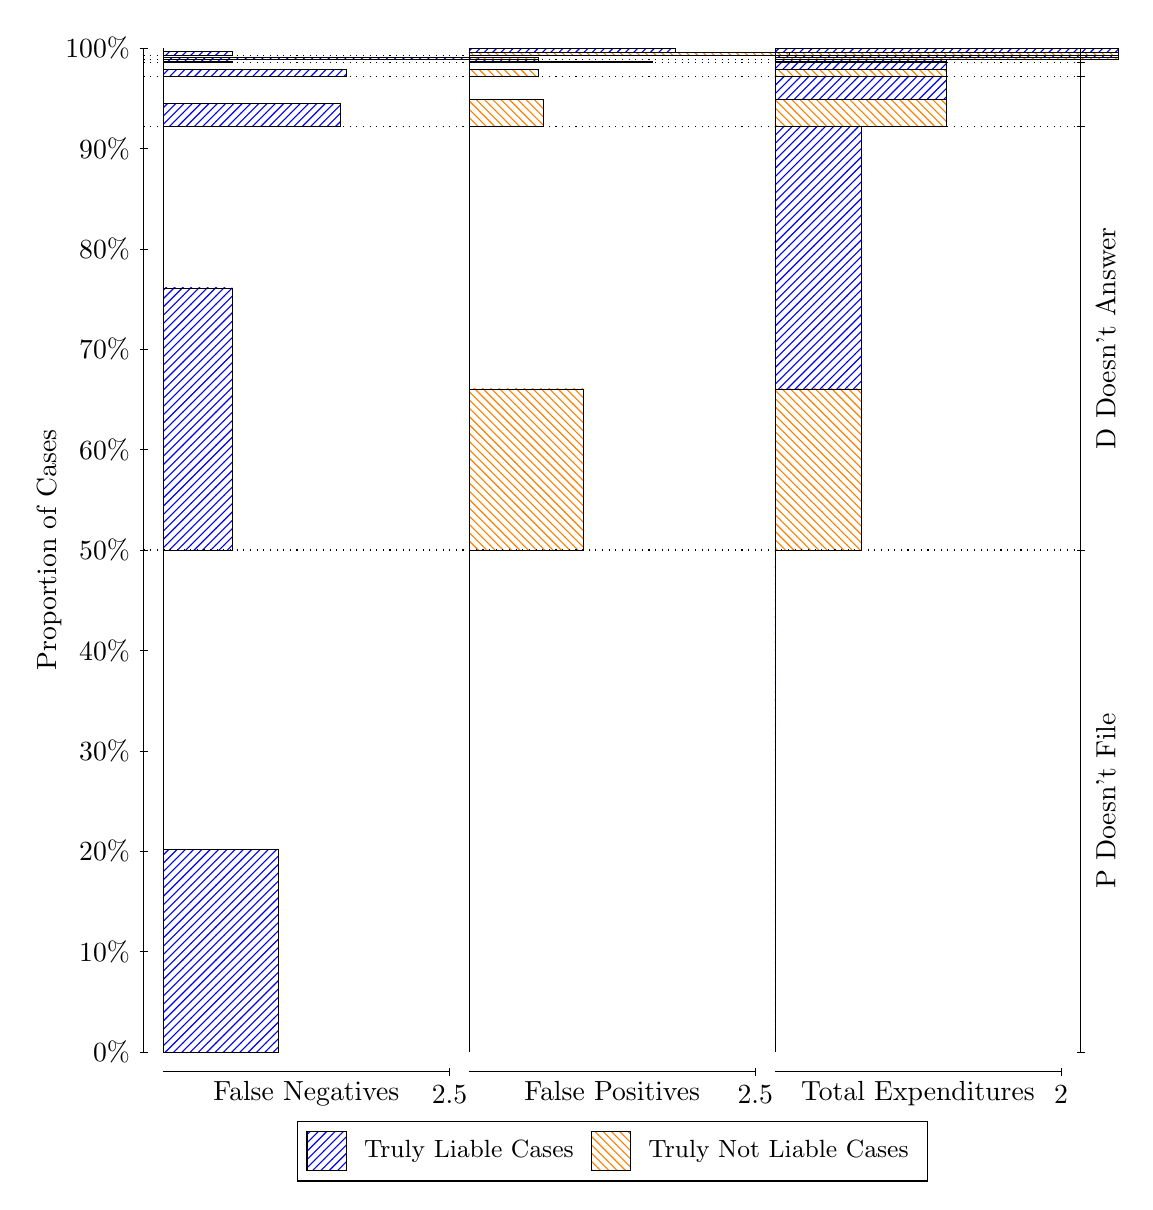
\begin{tikzpicture}
\draw[black, very thin] (1.5,1.75) -- (1.5,14.5);
\node[rotate=90, text=black, anchor=center] at (0.3, 8.125) {Proportion of Cases};
\draw[black, very thin] (1.45,1.75) -- (1.55,1.75);
\node[text=black, anchor=east] at (1.45, 1.75) {0\%};
\draw[black, very thin] (1.45,3.025) -- (1.55,3.025);
\node[text=black, anchor=east] at (1.45, 3.025) {10\%};
\draw[black, very thin] (1.45,4.3) -- (1.55,4.3);
\node[text=black, anchor=east] at (1.45, 4.3) {20\%};
\draw[black, very thin] (1.45,5.575) -- (1.55,5.575);
\node[text=black, anchor=east] at (1.45, 5.575) {30\%};
\draw[black, very thin] (1.45,6.85) -- (1.55,6.85);
\node[text=black, anchor=east] at (1.45, 6.85) {40\%};
\draw[black, very thin] (1.45,8.125) -- (1.55,8.125);
\node[text=black, anchor=east] at (1.45, 8.125) {50\%};
\draw[black, very thin] (1.45,9.4) -- (1.55,9.4);
\node[text=black, anchor=east] at (1.45, 9.4) {60\%};
\draw[black, very thin] (1.45,10.675) -- (1.55,10.675);
\node[text=black, anchor=east] at (1.45, 10.675) {70\%};
\draw[black, very thin] (1.45,11.95) -- (1.55,11.95);
\node[text=black, anchor=east] at (1.45, 11.95) {80\%};
\draw[black, very thin] (1.45,13.225) -- (1.55,13.225);
\node[text=black, anchor=east] at (1.45, 13.225) {90\%};
\draw[black, very thin] (1.45,14.5) -- (1.55,14.5);
\node[text=black, anchor=east] at (1.45, 14.5) {100\%};

\draw[black, very thin] (13.4,1.75) -- (13.4,14.5);
\draw[black, very thin] (13.35,1.75) -- (13.45,1.75);
\node[anchor=west] at (13.35, 1.75) {};
\draw[black, very thin] (13.35,8.1251) -- (13.45,8.1251);
\node[anchor=west] at (13.35, 8.1251) {};
\draw[black, very thin] (13.35,13.502) -- (13.45,13.502);
\node[anchor=west] at (13.35, 13.502) {};
\draw[black, very thin] (13.35,14.142) -- (13.45,14.142);
\node[anchor=west] at (13.35, 14.142) {};
\draw[black, very thin] (13.35,14.318) -- (13.45,14.318);
\node[anchor=west] at (13.35, 14.318) {};
\draw[black, very thin] (13.35,14.353) -- (13.45,14.353);
\node[anchor=west] at (13.35, 14.353) {};
\draw[black, very thin] (13.35,14.41) -- (13.45,14.41);
\node[anchor=west] at (13.35, 14.41) {};
\draw[black, very thin] (13.35,14.5) -- (13.45,14.5);
\node[anchor=west] at (13.35, 14.5) {};

\draw[black, very thin, pattern color=blue, pattern=north east lines] (1.75,1.75) rectangle (3.2033,4.3182);
\draw[black, very thin, pattern color=orange, pattern=north west lines] (1.75,4.3182) rectangle (1.75,8.1251);
\draw[black, very thin, pattern color=blue, pattern=north east lines] (1.75,8.1251) rectangle (2.622,11.455);
\draw[black, very thin, pattern color=orange, pattern=north west lines] (1.75,11.455) rectangle (1.75,13.502);
\draw[black, very thin, pattern color=blue, pattern=north east lines] (1.75,13.502) rectangle (4.0027,13.793);
\draw[black, very thin, pattern color=orange, pattern=north west lines] (1.75,13.793) rectangle (1.75,14.142);
\draw[black, very thin, pattern color=blue, pattern=north east lines] (1.75,14.142) rectangle (4.0753,14.229);
\draw[black, very thin, pattern color=orange, pattern=north west lines] (1.75,14.229) rectangle (1.75,14.318);
\draw[black, very thin, pattern color=blue, pattern=north east lines] (1.75,14.318) rectangle (2.622,14.338);
\draw[black, very thin, pattern color=orange, pattern=north west lines] (1.75,14.338) rectangle (1.75,14.353);
\draw[black, very thin, pattern color=blue, pattern=north east lines] (1.75,14.353) rectangle (5.8193,14.381);
\draw[black, very thin, pattern color=orange, pattern=north west lines] (1.75,14.381) rectangle (1.75,14.41);
\draw[black, very thin, pattern color=blue, pattern=north east lines] (1.75,14.41) rectangle (2.622,14.461);
\draw[black, very thin, pattern color=orange, pattern=north west lines] (1.75,14.461) rectangle (1.75,14.5);
\draw[black, very thin, pattern color=orange, pattern=north west lines] (5.6333,1.75) rectangle (5.6333,5.557);
\draw[black, very thin, pattern color=blue, pattern=north east lines] (5.6333,5.557) rectangle (5.6333,8.1251);
\draw[black, very thin, pattern color=orange, pattern=north west lines] (5.6333,8.1251) rectangle (7.0867,10.172);
\draw[black, very thin, pattern color=blue, pattern=north east lines] (5.6333,10.172) rectangle (5.6333,13.502);
\draw[black, very thin, pattern color=orange, pattern=north west lines] (5.6333,13.502) rectangle (6.578,13.851);
\draw[black, very thin, pattern color=blue, pattern=north east lines] (5.6333,13.851) rectangle (5.6333,14.142);
\draw[black, very thin, pattern color=orange, pattern=north west lines] (5.6333,14.142) rectangle (6.5053,14.231);
\draw[black, very thin, pattern color=blue, pattern=north east lines] (5.6333,14.231) rectangle (5.6333,14.318);
\draw[black, very thin, pattern color=orange, pattern=north west lines] (5.6333,14.318) rectangle (7.9587,14.333);
\draw[black, very thin, pattern color=blue, pattern=north east lines] (5.6333,14.333) rectangle (6.5053,14.353);
\draw[black, very thin, pattern color=orange, pattern=north west lines] (5.6333,14.353) rectangle (6.5053,14.382);
\draw[black, very thin, pattern color=blue, pattern=north east lines] (5.6333,14.382) rectangle (5.6333,14.41);
\draw[black, very thin, pattern color=orange, pattern=north west lines] (5.6333,14.41) rectangle (9.7027,14.449);
\draw[black, very thin, pattern color=blue, pattern=north east lines] (5.6333,14.449) rectangle (8.2493,14.5);
\draw[black, very thin, pattern color=orange, pattern=north west lines] (9.5167,1.75) rectangle (9.5167,5.557);
\draw[black, very thin, pattern color=blue, pattern=north east lines] (9.5167,5.557) rectangle (9.5167,8.1251);
\draw[black, very thin, pattern color=orange, pattern=north west lines] (9.5167,8.1251) rectangle (10.607,10.172);
\draw[black, very thin, pattern color=blue, pattern=north east lines] (9.5167,10.172) rectangle (10.607,13.502);
\draw[black, very thin, pattern color=orange, pattern=north west lines] (9.5167,13.502) rectangle (11.697,13.851);
\draw[black, very thin, pattern color=blue, pattern=north east lines] (9.5167,13.851) rectangle (11.697,14.142);
\draw[black, very thin, pattern color=orange, pattern=north west lines] (9.5167,14.142) rectangle (11.697,14.231);
\draw[black, very thin, pattern color=blue, pattern=north east lines] (9.5167,14.231) rectangle (11.697,14.318);
\draw[black, very thin, pattern color=orange, pattern=north west lines] (9.5167,14.318) rectangle (11.697,14.333);
\draw[black, very thin, pattern color=blue, pattern=north east lines] (9.5167,14.333) rectangle (11.697,14.353);
\draw[black, very thin, pattern color=orange, pattern=north west lines] (9.5167,14.353) rectangle (13.877,14.382);
\draw[black, very thin, pattern color=blue, pattern=north east lines] (9.5167,14.382) rectangle (13.877,14.41);
\draw[black, very thin, pattern color=orange, pattern=north west lines] (9.5167,14.41) rectangle (13.877,14.449);
\draw[black, very thin, pattern color=blue, pattern=north east lines] (9.5167,14.449) rectangle (13.877,14.5);
\draw[black, dotted] (1.5,8.1251) -- (13.4,8.1251);
\draw[black, dotted] (1.5,13.502) -- (13.4,13.502);
\draw[black, dotted] (1.5,14.142) -- (13.4,14.142);
\draw[black, dotted] (1.5,14.318) -- (13.4,14.318);
\draw[black, dotted] (1.5,14.353) -- (13.4,14.353);
\draw[black, dotted] (1.5,14.41) -- (13.4,14.41);
\draw[black, very thin] (1.75,1.5) -- (5.3833,1.5);
\node[text=black, anchor=north] at (3.5667, 1.5) {False Negatives};
\draw[black, very thin] (5.3833,1.45) -- (5.3833,1.55);
\node[text=black, anchor=north] at (5.3833, 1.45) {2.5};

\draw[black, very thin] (5.6333,1.5) -- (9.2667,1.5);
\node[text=black, anchor=north] at (7.45, 1.5) {False Positives};
\draw[black, very thin] (9.2667,1.45) -- (9.2667,1.55);
\node[text=black, anchor=north] at (9.2667, 1.45) {2.5};

\draw[black, very thin] (9.5167,1.5) -- (13.15,1.5);
\node[text=black, anchor=north] at (11.333, 1.5) {Total Expenditures};
\draw[black, very thin] (13.15,1.45) -- (13.15,1.55);
\node[text=black, anchor=north] at (13.15, 1.45) {2};

\node[text=black, centered, rotate=90] at (13.72, 4.9376) {P Doesn't File};
\node[text=black, centered, rotate=90] at (13.72, 10.813) {D Doesn't Answer};






\draw (7.449999999999999,1.5) node[draw=none] (baseCoordinate) {};
\begin{scope}[align=center]
        \matrix[scale=0.5, draw=black, below=0.5cm of baseCoordinate, nodes={draw}, column sep=0.1cm]{
            \node[rectangle, draw, minimum width=0.5cm, minimum height=0.5cm, pattern color=blue, pattern=north east lines] {}; &
            \node[draw=none, font=\small, text=black] (B) {Truly Liable Cases}; &
            \node[rectangle, draw, minimum width=0.5cm, minimum height=0.5cm, pattern color=orange, pattern=north west lines] {}; &
            \node[draw=none, font=\small, text=black] (B) {Truly Not Liable Cases}; \\
            };
\end{scope}

\end{tikzpicture}
\end{document}